\documentclass[10pt, a4paper, twocolumn]{jarticle}
%\documentclass[10pt, a4paper, twocolumn, uplatex]{jsarticle}
\usepackage{proceeding_bachelor}
\usepackage{tabularx}
\usepackage{booktabs}
\usepackage{multirow}
\usepackage{cite}
\usepackage{amsmath, amssymb}
\usepackage{svg}

% Title info. ======================================
\title{不確実性適応型損失関数による \\
頑健な医用画像セグメンテーション}

%%%%% 著者 %%%%%
\author{廣池 友哉}

%%%% 学籍番号 %%%%
\studentid{M243422}

%%%% 所属 %%%%
\affiliation{広島大学 大学院先進理工系科学研究科 情報科学プログラム}

%%%% 年度を書き換える %%%%
\proceedingname{2025年度修士論文中間発表予稿}

%%%% 卒論発表の日付を書く %%%%
\date{2025/9/19}


\begin{document}
%%%%%%%%%%%%% Header and Title %%%%%%%%%%%%%
\maketitle


%%% Please write your body text from here %%
\section{はじめに}
医用画像セグメンテーションは,診断支援や治療計画において不可欠な技術であり,
正常組織または異常組織の領域を抽出ことが求められる.
特に大腸ポリープ\cite{ji2022video}や頭頸部がん放射線治療における危険臓器\cite{maleki2020machine}の検出など,臨床応用が進んでいる.

しかしながら,医用画像セグメンテーションは固有の課題が存在する.特に重要な問題として,クラス不均衡が挙げられる.
医用画像では背景領域が大部分を占め,対象となる病変は相対的に小さい領域しか占めないことが多い.
この状況下では,従来の分類タスクで広く使われているCross-Entropy Loss\cite{long2015fully}は背景領域の学習に偏り,
臨床的に重要な小病変や曖昧な境界部分の正確なセグメンテーションが困難となる.

この課題に対処するため,クラス不均衡に対して頑健なDice Loss\cite{milletari2016v}やその
多くの拡張手法が提案され,CT画像\cite{zhu2019anatomynet, 9109297}や
MRI画像\cite{KATO2024107695}において高い性能が報告されている.
しかし,これらのアプローチでは損失関数は全画像に対して固定的な形状を持つという制約がある.医用画像の多様性を考慮すると,
画像ごとの難易度に応じて損失関数を適応的に調整することが望ましい.
このような適応的学習を実現するためには,損失関数の形状を制御する機構と,各画像の難易度を定量化する仕組みの2つが必要である.
検出難易度が高い画像に対する学習が不十分になり,頑健な検出が困難であるという課題がある.

本研究では,これら2つの要素を組み合わせた適応的学習フレームワークの構築を目指す.
形状制御には,Dice Lossを多項式展開して得られるPolyDice Lossを用いる.
難易度の定量化には,Monte Carlo Dropout\cite{pmlr-v48-gal16}(以下,MC Dropout)による
推定を用いる.MC Dropoutは推論時にDropoutを有効にすることで,モデルの認識的不確実性を効率的に推定し,
モデルが各画像をどの程度「難しい」と感じているかを定量化できる.
本稿では,この最終目標に向けた第一段階として,ピクセル単位の不確実性指標が学習過程でどのように推移するかを分析し,
画像難易度の定量化手法としての妥当性を評価する.
\section{提案法}

\subsection{概要}
本研究の最終目標は,画像ごとのセグメンテーション難易度を学習中に動的に評価し,
その難易度に応じて損失関数の形状を適応的に変化させるシステムの構築である.
図に提案法の全体構成を示す.
提案法では,学習中各画像に対してMC Dropoutを用いて画像毎に複数枚推論を行い,予測のばらつきから不確実性を定量化する.
この不確実性情報は,モデルがその画像のセグメンテーションをどの程度「難しい」と感じているかを反映する.
将来的には,この不確実性情報を画像単位に集約し,PolyDice Lossの形状を動的に制御することで,
難しい画像には急峻な勾配を,簡単な画像には緩やかな勾配を与える適応的学習を実現する.

本稿では,最終目標に向けた基礎的検証として,ピクセル単位の不確実性指標が学習過程でどのように推移するかを分析し,
画像難易度の指標としての妥当性を検証する.

\subsection{PolyDice Lossによる損失形状制御}
医用画像セグメンテーションで広く使用されるDice Lossは,クラス不均衡に頑健であるが,全画像に対して固定的な形状を持つという制約がある.
本研究では,Dice Lossを多項式展開により拡張したPolyDice Loss [引用],特にその実用的な形式であるPolyDice-1 Lossを採用する.
PolyDice-1 Lossは,単一のパラメータ$\epsilon$で損失関数の形状を制御でき,画像の難易度に応じて勾配の急峻さを調整することが可能となる.

\subsubsection{Dice Loss}
画像サイズを $H \times W$とし,ピクセル位置を $(i, j)$ で表す$\left(i \in \{1, ..., H\}, j \in \{1, ..., W\}\right)$.
セグメンテーションタスクにおいて,モデルの予測確率マップを$\hat{\mathbf{Y}} = \{\hat{y}_{i,j}\}_{i,j} \in \mathbb R ^ {H \times W}$,
その画像に対する正解マスクを$\mathbf{Y} = \{{y}_{i,j}\}_{i,j} \in \mathbb R ^ {H \times W}$とすると,Dice Lossは次式で定義される.

\begin{equation}
  \mathcal{L}_{\text{Dice}}(\hat{\mathbf{y}}, \mathbf{y}) = 1 - \frac{2 \sum_{i=1}^{W} \sum_{j=1}^{H} \hat{y}_{i, j} y_{i, j}}{\sum_{i=1}^{W} \sum_{j=1}^{H}(\hat{y_{i, j}} ^ 2 + y_{i, j} ^ 2)}
\end{equation}

\subsubsection{幾何学的解釈と多項式展開}

予測確率マップ$\hat{\mathbf{Y}}$と正解マスク$\mathbf{Y}$をそれぞれ長さ$HW$のベクトル$\hat{\mathbf{Y}}, \mathbf{Y}$
として平坦化すると,Dice Lossは以下のように分解できる.

\begin{equation}
  \mathcal{L}_{\text{Dice}} = 1 - s \cos  \theta
\end{equation}
% \begin{equation}
%   \begin{aligned}
%     \mathcal{L}_{\text{Dice}} &= 1 - \frac{2 \langle \hat{\mathbf{y}} ^ {\prime}, {\mathbf{y}} ^ {\prime} \rangle}{\Vert \hat{\mathbf{y}} ^ {\prime} \Vert ^ 2 + \Vert {\mathbf{y}} ^ {\prime} \Vert ^ 2} \\
%     &= 1 - \frac{2 \Vert \hat{\mathbf{y}} ^ {\prime} \Vert \Vert {\mathbf{y}} ^ {\prime} \Vert}{\Vert \hat{\mathbf{y}} ^ {\prime} \Vert ^ 2 + \Vert {\mathbf{y}} ^ {\prime} \Vert ^ 2}
%     \times \frac{\langle \hat{\mathbf{y}} ^ {\prime}, {\mathbf{y}} ^ {\prime} \rangle}{\Vert \hat{\mathbf{y}} ^ {\prime} \Vert \Vert {\mathbf{y}} ^ {\prime} \Vert}
%   \end{aligned}
% \end{equation}
ここで,$s = \frac{2 \langle \hat{\mathbf{y}} ^ {\prime}, {\mathbf{y}} ^ {\prime} \rangle}{\Vert \hat{\mathbf{y}} ^ {\prime} \Vert ^ 2 + \Vert {\mathbf{y}} ^ {\prime} \Vert ^ 2}$はスケール成分,
$\theta = \frac{\langle \hat{\mathbf{y}} ^ {\prime}, {\mathbf{y}} ^ {\prime} \rangle}{\Vert \hat{\mathbf{y}} ^ {\prime} \Vert \Vert {\mathbf{y}} ^ {\prime} \Vert}$は2つの
ベクトル間の角度を表す.この分解により,Dice Lossはスケール成分$s$と$\cos \theta$の積として理解できる.

方向成分$\cos \theta$に対してTaylor展開を適用することで,PolyDice Lossの多項式表現を導出する.
つまり$\theta \approx 0$(予測と正解が大きく異ならない)と仮定し,$\cos{\theta}$を$\theta = 0$まわりでテイラー展開すると以下のように近似できる.
\begin{equation}
  \cos{\theta} = 1 - \frac{\theta ^ 2}{2!} + \frac{\theta ^ 4}{4!} - \cdots
\end{equation}
これをDice Lossに代入し,整理するとPolyDiceの一般形が得られる:
% \begin{equation}
%   \begin{aligned}
%   \mathcal{L}_{\text{Dice}} &= 1 - s \left(1 + \frac{1}{2!} \theta ^ 2 - \frac{1}{4!} \theta ^ 4 + \cdots\right) \\
%   &= (1 - s) + s \left[\sum_{k = 1}^{\infty} \frac{(-1) ^ {k - 1}}{(2k)!} \theta ^ {2k}\right]
% \end{aligned}
% \end{equation}
\begin{equation}
  \mathcal{L}_{\text{PolyDice}} = (1 - s) + s \sum_{k = 1}^{\infty} \alpha_k \theta ^ {2k}
\end{equation}
ここで, $\alpha_k=\frac{(-1)^{k-1}}{(2k)!}$は各Taylor項の符号係数である.

% この損失関数を計算するために、角度$\theta$は以下のようにコサインの逆関数を用いて算出される.
% \begin{equation}
%   \theta = \arccos{\left(\frac{\langle \hat{\mathbf{y}} ^ {\prime}, {\mathbf{y}} ^ {\prime} \rangle}{\Vert \hat{\mathbf{y}} ^ {\prime} \Vert \Vert {\mathbf{y}} ^ {\prime} \Vert}\right)}
% \end{equation}

\subsubsection{PolyDice-1 Loss}
実用的な観点から,\cite{leng2022polyloss}のアプローチに従い,第$1$項のみを調整可能とするPolyDice-1 Lossを採用する:
\begin{equation}
  \mathcal{L}_{\text{PolyDice-1}} = (1 - s) + s \left(\frac{1}{2} + \epsilon\right) \theta^2
\end{equation}
ここで,$\epsilon \in \mathbb{R}$は損失関数の形状を制御するハイパーパラメータである.
図\ref{polydice}に,$\epsilon$に応じたPolyDice-1 Lossの形状変化を示す.
$\epsilon > 0$では予測誤差に対するペナルティが強化され,$\epsilon < 0$では緩和される.
本稿では,まず$\epsilon = 0$で固定して実験を行い,将来的にはこの$\epsilon$を不確実性に基づいて動的に調整する.

\begin{figure}
  \includegraphics[scale=0.25]{figure/loss.pdf}
  \caption{Plot of PolyDice-1 Loss($s = 0.1$)}
  \label{polydice}
\end{figure}

\subsection{不確実性による難易度評価}

\subsubsection{MC Dropoutの原理と適用}

Dropoutは元々,ニューラルネットワークの過学習を防ぐ正則化手法として提案された [引用:Srivastava et al., 2014].
訓練時に各層のニューロンを確率$p$でランダムに不活性化することで
モデルの汎化性能を向上させる.通常,推論時にはDropoutは無効化され,全ニューロンが活性化される.

MC Dropoutは.学習時のみだけでなく,推論時にもDropoutを有効にすることで,モデルの認識的不確実性を推定する手法である.
通常,推論時の出力は決定論的であるが,Dropoutを有効にすることで,
異なるサブネットワークが形成され、確率的な出力が得られる.
同一入力に対してこの確率的な推論を複数回実行して得られる予測結果の分布は、
Bayesian Neural Networkにおける予測事後分布近似とみなせ,変分推論の一種として解釈できる.

提案法では,このMC Dropoutを学過程の各段階で適用する.
具体的には,$\tau$エポックごとに推論フェーズを挿入し,その時点でのモデルが各セグメンテーションをどの程度「難しい」と感じているかを定量化する.
% これにより,学習の進行に伴う不確実性の時系列変化を追跡できる.てDropoutを確率$p$でMC Dropoutを$N$回実行することで,
% 各学習段階で$N$枚の複数の予測画像を得る.
% またDropout層はモデルの最も深いエンコーダおよびデコーダに配置する.
% 浅い層と比較してより高次な特徴を抽出する深い層でDropoutを実行することで,
% 高次な意味的判断におけるモデルの確信度がより直接的に反映されることが期待される.

\subsubsection{学習中のMC Dropout推論}
学習エポック$e \in \{\tau, 2\tau, \ldots, E\}$において,次の手順で不確実性評価を実施する.
セグメンテーション学習済みモデル$f_{\theta}: \mathcal{X} \rightarrow [0,1]^{H \times W}$に対し,Dropout率$p \in (0,1)$で
エポック$e$時点のパラメータ$\theta^{(e)}$を固定する.
訓練データの各画像$x \in \mathcal{X}$に対して,
$N$回の確率的推論を行い,予測集合$\{\hat{Y}^{(n)}\}_{n=1}^{N}$を得る:
%
\begin{equation}
  \hat{\mathbf{Y}}^{(n)} = f_{\theta^{(e)}}(x; \mathbf{z}^{(n)}), \quad \mathbf{z}^{(n)} \sim \text{Bernoulli}(1-p)
\end{equation}
%
ここで,$\mathbf{z}^{(n)}$は$n$回目の推論におけるDropoutマスク(各ニューロンの活性/非活性を決定),
各$\hat{\mathbf{Y}}^{(n)} = \{\hat{y}_{i,j}^{(n)} \in [0,1]\}_{i,j}$は$n$回目の推論における予測確率マップである.
この確率的推論により,同一画像に対して複数の予測マップが得られ,
そのばらつきから「モデルがどれだけ迷っているか」を定量化可能である.

\subsubsection{ピクセル単位の不確実性指標の計算}
得られた$N$枚の予測画像に対し,ピクセル単位で不確実性指標を計算する.
不確実性マップから,以下の3つの不確実指標をピクセル単位で計算する.

\begin{itemize}
  \item \textbf{予測分散}:
  \begin{equation}
    \text{Var}(\hat{y}_{ij}) = \frac{1}{N} \sum_{n=1}^{N} (\hat{y}_{ij}^{(n)} - \bar{y}_{i,j})^2
  \end{equation}
  ここで,$\bar{y}_{i,j} = \frac{1}{N} \sum_{k = 1}^{N} \hat{y}_{ij} ^ {(n)}$は予測の平均である.
  この指標は,複数回の予測がどの程度ばらついているかを表し,値が大きいほどモデルの予測が不安定であることを示す.
  \item \textbf{予測エントロピー}:
  \begin{equation}
    H(\bar{y}_{i,j}) = - \bar{y}_{i,j} \log{\bar{y}_{i,j}} - (1 - \bar{y}_{i,j}) \log{(1 - \bar{y}_{i,j})}
  \end{equation}
  これは平均予測の不確実性を表す.エントロピーは予測確率が$0.5$に近いほど高くなり,
  モデルが前景・背景の判断に迷っていることを示す.確率が$0$または$1$に近い場合は低い値となる.
  \item \textbf{相互情報量}:
  \begin{equation}
    I(y_{ij}) = H(\bar{\hat{y}}_{ij}) - \frac{1}{N}\sum_{n=1}^{N} H(\hat{y}_{ij}^{(n)})
  \end{equation}
  これはモデルパラメータの不確実性(認識的不確実性)を表す.
  全体の不確実性から偶然的不確実性を引いたもので,より多くのデータで学習することで減少する性質を持つ.
  この値が高い領域は,モデルが十分に学習できていない可能性を示唆する.
\end{itemize}

\subsection{画像全体の難易度への集約と適応的制御(将来構想)}

\subsubsection{画像単位への集約}
ピクセル単位の不確実性マップ$\mathbf{U} = \{u_{i,j}\}_{i,j}$から画像全体の難易度スコア$D \in \mathbb{R}^+$を算出する必要がある.
セグメンテーションタスクの特性を考慮すると,境界領域の不確実性に着目する方法や,予測誤差と相関の高い領域を重視する方法などが考えられる.
また,不確実性の空間的分布パターンや,前景・背景それぞれの不確実性の違いも重要な情報となる可能性がある.

\subsubsection{適応的パラメータ制御}
画像難易度スコア$D$に基づいて,Poly Dice Lossのパラメータ$\epsilon$を動的に制御する:

\begin{equation}
  \epsilon = g(D; \theta_g)
\end{equation}
ここで,$g$は制御関数,$\theta_g$はその学習可能なパラメータである.
難易度が高い画像には大きな$\epsilon$を割り当てて急峻な勾配を与え,
簡単な画像には小さな$\epsilon$で緩やかな勾配を与えることで,効率的な学習を実現する.

\section{実験}
\subsection{実験設定}
\subsubsection{データセット}
医用画像セグメンテーションにおける画像難易度の指標としての不確実性の妥当性を検証するため,CVC-ClinicDB\cite{BERNAL201599}データセットを用いて実験を行った.
本データセットは,$612$枚の大腸内視鏡画像($384 \times 288$ pixel)とそれに対応するポリープの正解マスクから構成される.
訓練データとテストデータの割合は$8:2$の比率で訓練・テストに分割し,訓練データの$10 \%$をランダムに抽出して検証データとした.
なお,本稿の予備的な解析では,このうち訓練データのみを使用して不確実性指標の推移を分析した.

\subsubsection{実装の詳細}
セグメンテーションモデルには$3$層のU-Net\cite{ronneberger2015u}を採用した.
学習にAdam optimizer\cite{kingma2014adam}を使用し,バッチサイズ$32$, 学習率$10 ^ {-3}$に設定した.
損失関数にはPolyDice-1 Loss($\epsilon = 0$)を用いた.
前処理として全画像を$W = 224$ pixel, $H = 224$ pixelにリサイズし,訓練時には
$50\%$の確率で上下左右反転および明度・コントラストの変更を施した.
最大エポック数は$200$に設定した.

MC Dropoutによる不確実評価は,$\tau=10$エポックごとに実施した.各評価時には,
$p = 0.5$で$N = 10$回の確率的推論を行い,ピクセル単位の不確実性指標を計算した.

\subsection{結果と考察}

\begin{figure}[t] % ← [t]をここに移動する
  \begin{center}
    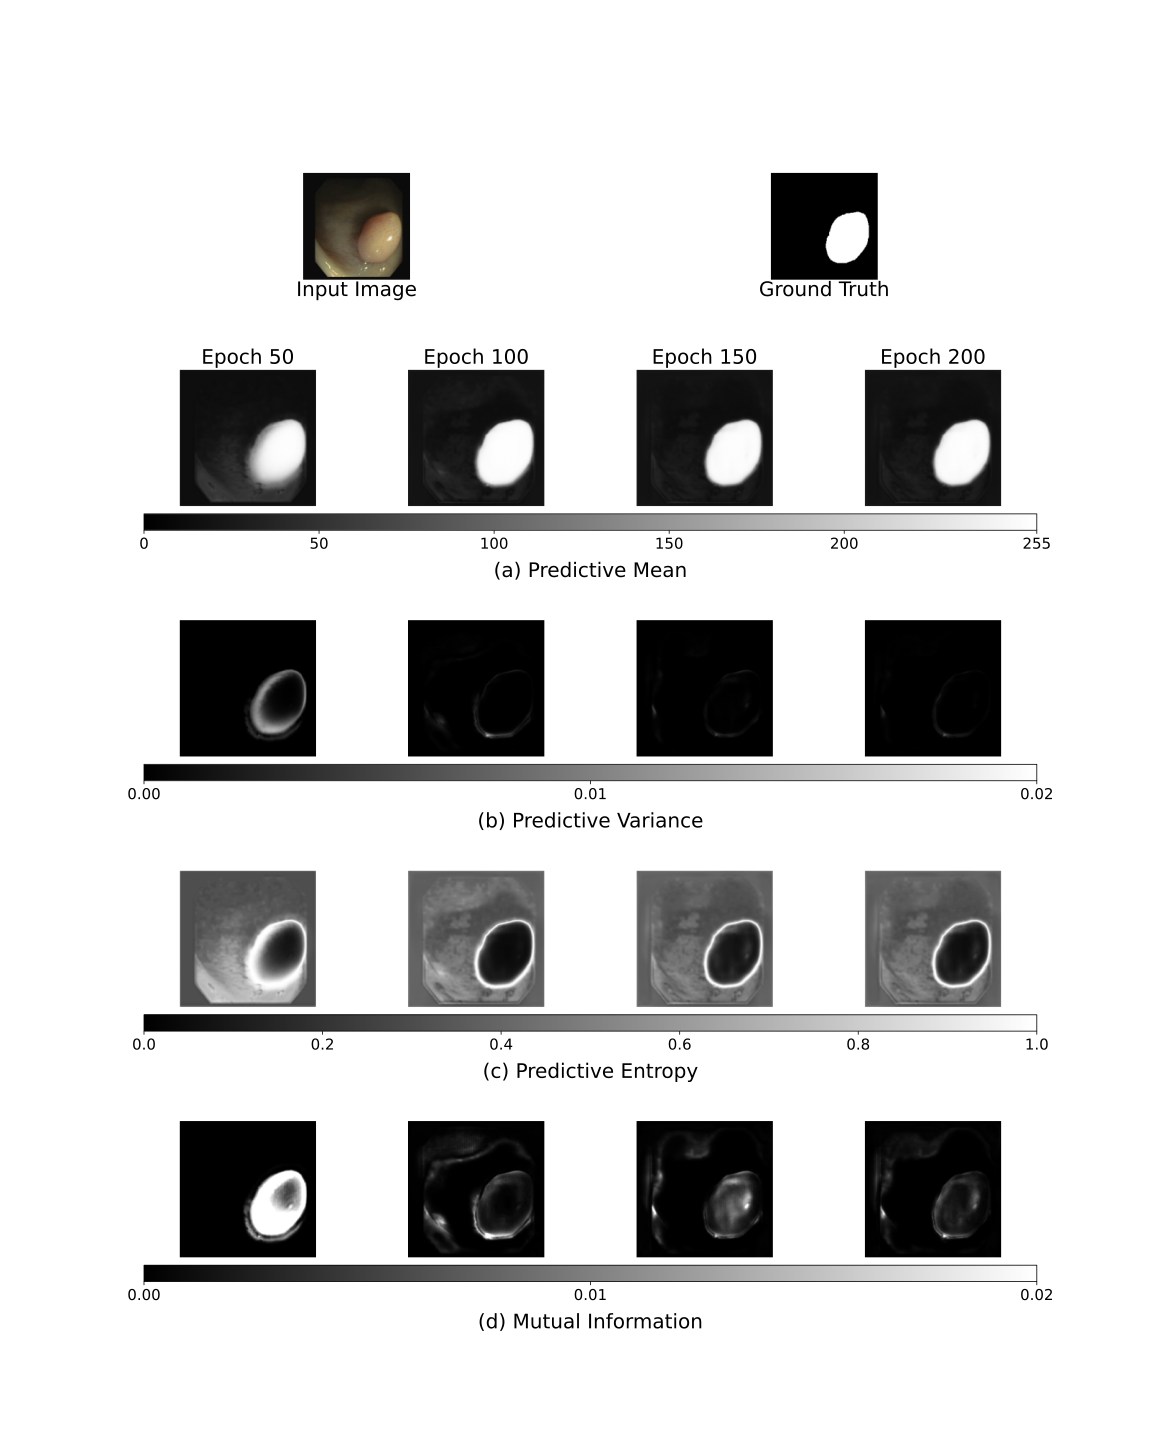
\includegraphics[width=\hsize]{figure/fold5_file144_uncertainty_evolution.pdf}
    \caption{Temporal evolution of uncertainty metrics for an easy case}
    \label{fold5_file144}
  \end{center}
\end{figure}

\begin{figure}[t] % ← [t]をここに移動する
  \begin{center}
    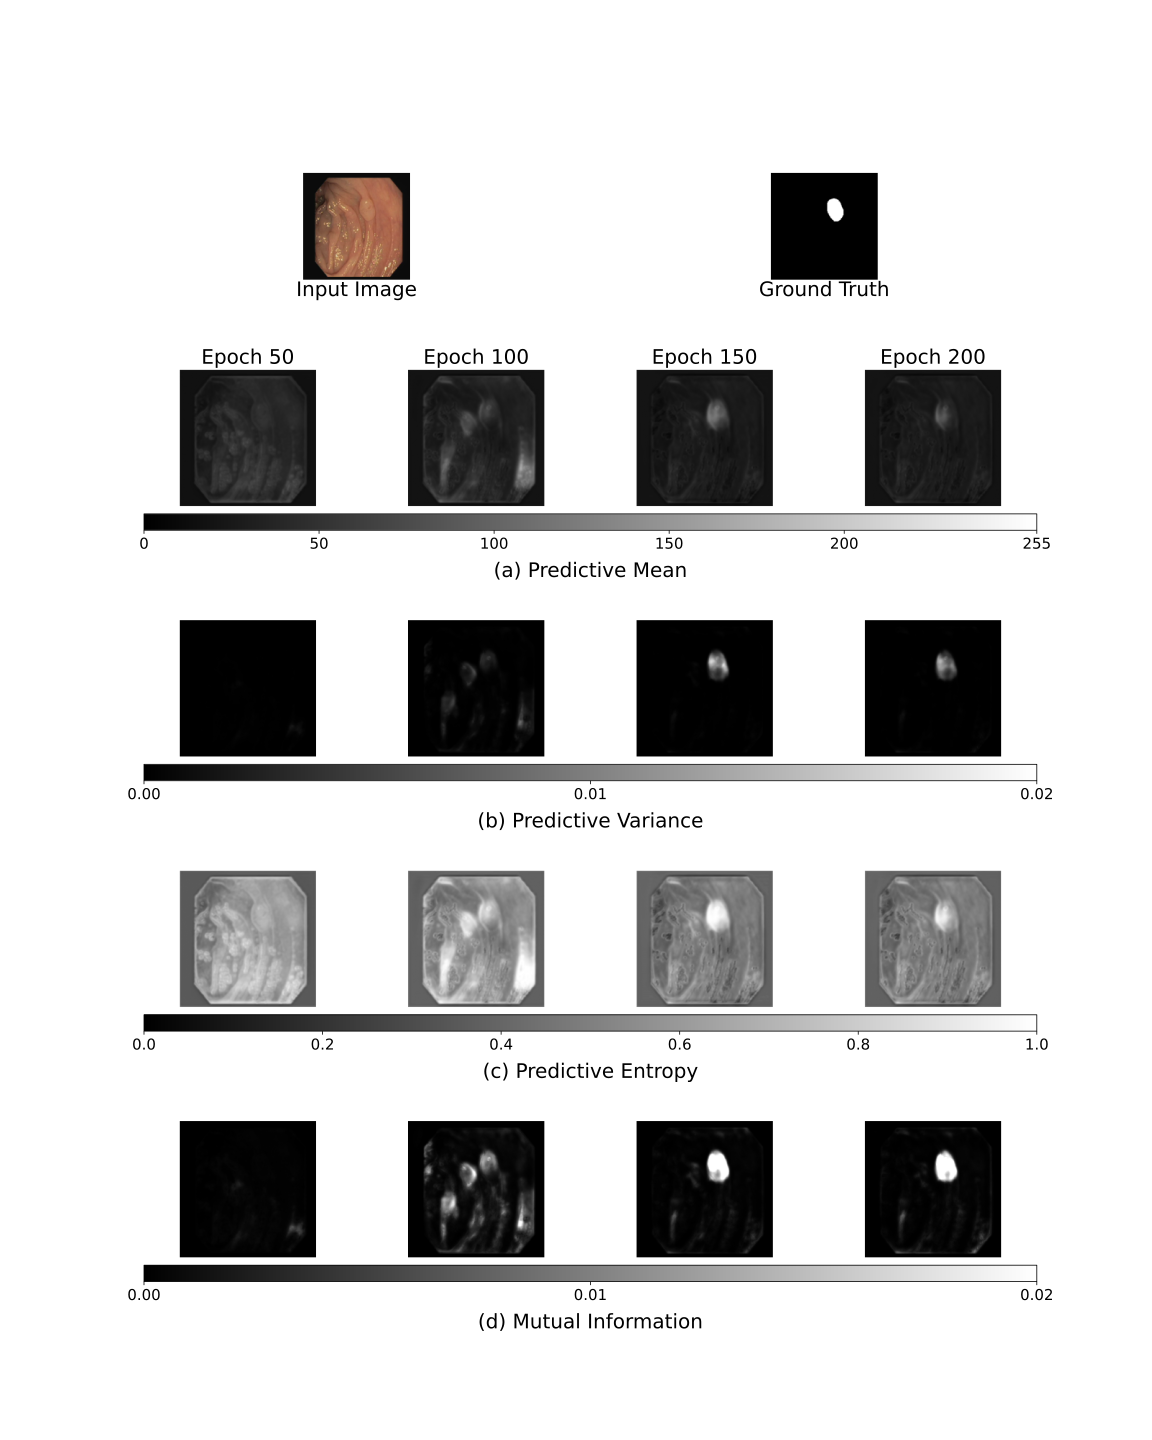
\includegraphics[width=\hsize]{figure/fold2_file450_uncertainty_evolution.pdf}
    \caption{Temporal evolution of uncertainty metrics for a difficult case}
    \label{fold2_file450}
  \end{center}
\end{figure}


\subsubsection{学習過程における不確実性の推移}
学習初期に高い精度で予測できるようになった画像群から代表例を1つ選択し($200$epoch時点でDice係数$0.981$,以下「簡単な例」),
学習後期においても精度が低い画像群から代表例を1つ選択し($200$epoch時点でDice係数$0$,以下「難しい例」),
それぞれの不確実指標の推移を分析した.図\ref{fold5_file144}に簡単な例,図\ref{fold2_file450}に難しい例の
$50, 100, 150, 200$ epoch時点での(b)予測分散,(c)予測エントロピー,(d)は相互情報量を示す.
参考として,MC Dropoutによる平均予測マップを(a)に併記している.
カラースケールは両例間で統一し,全ピクセル・全エポックにおける最大値で正規化した.

簡単な例では,予測平均(図\ref{fold5_file144}(a))が$50$エポック時点で既にポリープ領域を明確に捉えており,
とともに予測がより鮮明になった.予測分散(図\ref{fold5_file144}(b))と相互情報量(図\ref{fold5_file144}(d))は
学習の進行とともに急速に減少し,特に相互情報量は$100$エポック以降でほぼ消失した.これはモデルが早期に安定した特徴表現を獲得したことを示している.
一方,予測エントロピー(図1(c))はポリープ境界部で高い値を示し続け,境界の曖昧性が残存していることが分かる.

難しい例では,予測平均(図\ref{fold2_file450}(a))がポリープの正確な位置を捉えられず,$200$エポック時点でも高い予測スコアが得られていないことが観察された.
予測分散(図\ref{fold2_file450}(b))と相互情報量(図\ref{fold2_file450}(d))は,学習初期には低い値であったが,$100$エポック以降はポリープ領域に集中して高い値を示した.
特に相互情報量は$200$エポック時点でもポリープ中心部で高い値を維持しており,モデルが一貫した特徴表現を獲得できていないことを示している.
予測エントロピー(図\ref{fold2_file450}(c))は$50$エポック時点で画像全体に広がっていたが,学習の進行とともにポリープ領域に集約される傾向を示した.

\subsubsection{不確実性指標の比較分析}

今回の検証から,各不確実性指標が捉える「難しさ」の側面について,2つの代表例の結果を比較分析した.
相互情報量は,簡単な例では$100$エポック以降でほぼ$0$に収束したのに対し,難しい例では
ポリープ領域で高い値を維持し続けた.この差異は,相互情報量が
これらはモデルの知識不足に起因する偶然的不確実性を的確に捉えていることを示している.

一方,予測エントロピーは,学習が十分に進んだ後でも両例において境界部分で高い値を示し続けた.これは,
残存する「データ固有の曖昧さ」に起因するアレアトリック不確実性をを反映していると考えられる.
予測分散は相互情報量と類似した傾向を示したが,値のダイナミックレンジが小さく,症例間の差異が相互情報量ほど明確ではなかった.

\subsubsection{適応的損失関数への示唆}
本検証により,相互情報量が画像難易度の指標として最も妥当である可能性が示された.簡単な例では相互情報量が収束し,
難しい症例では学習後期でも高い値が残存するという対応関係が確認されたためである.この知見に基づき,相互情報量を
集約された難易度指標$D$の値が高い画像に対してはPolyDice-1 Lossのパラメータ$\epsilon$を増加させ,
急峻な勾配を与える制御が有効であると考えられる.

実装上の課題として,ピクセル単位の相互情報量を画像単位に集約する方法の設計が挙げられる.
本実験で観察された空間的分布,特に難しい例では
不確実性がポリープ内に広範囲に分布する傾向を考慮し,
正解マスク領域に着目した集約方法が有望である.これにより,病変検出の精度向上に直結する適応的学習の実現が期待される.

\section{まとめと今後の課題}
本稿では,医用画像セグメンテーションの誤差関数において,検出難易度が高い画像に対する学習が不十分になり,頑健な検出が困難であるという課題に対処するため,
検出難易度を画像毎に算出したものを学習に取り入れ,誤差関数の形状を動的に変化させる手法を提案した.
提案法では,学習中各画像に対してMC Dropoutを用いて画像毎に複数枚推論を行い,
予測のばらつきから不確実性を定量化した.
医用画像データセットを用いた実験の結果,学習後期においても精度が低い症例に関して,
ピクセル単位の相互情報量の分散と相互情報量が増大していくことが明らかになった.
今後は,上記の不確実性指標を領域周辺に着目して集約する方法を検討し,
難易度が高い画像には急峻な勾配を与えることで,精度が低い症例でも頑健な検出を実現できる
制御関数を実装し,提案法の有効性を検証する予定である.

%%%%% 参考文献(BibTeXを使う場合) %%%%%
\bibliographystyle{bibstyle} % bstファイルを設定
\bibliography{references} % bibファイルを読み込み

%%%%% 参考文献(直接書く場合) %%%%%
% \begin{thebibliography}{9} %\footnotesize
    % \bibitem{kajiya1986rendering}
    % J.~T. Kajiya,
    % \newblock ``The rendering equation,''
    % \newblock in {\em Proceedings of the 13th Annual Conference on Computer
    %   Graphics and Interactive Techniques}, pp. 143--150, 1986.
    
    % \bibitem{jensen2001realistic}
    % H.~W. Jensen,
    % \newblock {\em Realistic image synthesis using photon mapping}, vol. 364,
    % \newblock Ak Peters Natick, 2001.
% \end{thebibliography}

% ★★★ ここに表を移動 ★★★
\clearpage % 改ページして、これまでのフロート(図表)をすべて出力

\begin{table*}[htb]
  \centering
  \caption{U-Netモデルのアーキテクチャ概要}
  \label{tab:unet_architecture}
  \begin{tabular}{lcc}
    \toprule
    \textbf{層 (Layer)} & \textbf{出力形状 (H x W x C)} & \textbf{備考 (Notes)} \\
    \midrule
    \multicolumn{3}{c}{\textit{--- Encoder ---}} \\
    Input & 224 x 224 x 3 & 入力画像 \\
    inc (DoubleConv) & 224 x 224 x 64 & \\
    down1 (MaxPool + DoubleConv) & 112 x 112 x 128 & \\
    down2 (MaxPool + DoubleConv) & 56 x 56 x 256 & \\
    down3 (MaxPool + DoubleConv) & 28 x 28 x 512 & \\
    down4 (MaxPool + DoubleConv) & 14 x 14 x 512 & ボトルネック, Dropout適用 \\
    \midrule
    \multicolumn{3}{c}{\textit{--- Decoder ---}} \\
    up1 (Upsample + DoubleConv) & 28 x 28 x 256 & Skip conn. from down3, Dropout適用 \\
    up2 (Upsample + DoubleConv) & 56 x 56 x 128 & Skip conn. from down2 \\
    up3 (Upsample + DoubleConv) & 112 x 112 x 64 & Skip conn. from down1 \\
    up4 (Upsample + DoubleConv) & 224 x 224 x 64 & Skip conn. from inc \\
  \midrule
  outc (Conv2d) & 224 x 224 x 2 & 出力 (2クラス) \\
  \bottomrule
  \end{tabular}
\end{table*}


\end{document}